\chapter{Introduction}
\label{label:chapIntro}

\section{The Standard Model}
A physics model is a description of a system using physics and mathematical concepts and language.
Standard Model (SM) is a physics model that summarizes what is known in the subatomic world. 
In SM, there are 
two types of fundamental particles, fermions and bosons. Fundamental fermions are the building block of matter,
and fundamental bosons are the intermediate particles of the four fundamental interactions of SM, i.e., strong, weak, electromagnetic and
gravitational force. 
In this chapter, we will briefly introduce the components of the SM and the related theories to the my thesis. 
A detailed elaboration about the SM could be found in books like Griffiths~\cite{particlebook1}. 

\subsection{Fundamental particles}

Fermions are defined as particles with half integer spin (intrinsic angular momentum), for example lepton, quark, proton, etc. 
%Note even composite particles, like proton and neutron, are also fermions.  
While bosons are particles with integer spin, like photon and Higgs boson.
The fundamental particles of SM are shown in Figure~\ref{figs:SMParticles}. 


{\bf Quarks}

In SM, there are six flavors of quarks: up (u), down (d), strange (s), charm (c), top (t) and bottom (b).  
Quarks carry properties like flavor, color, spin, charge, mass, etc and they belong to one of the three generations. 
u and d quarks belong to the first generation; s and c quarks are the second generation quarks; t and b quarks 
make up the third generation. The generation of quarks is mostly categorized by their coupling strength with each other in 
the weak interactions and also their discovery time.  
The color of quarks, arising from the Quantum Chromodynamics, is a property to be conserved in strong interactions. 
There are normally 3 types of color: red, blue, green. A particle is colorless if it carries a net color 
charge of zero. 
All quarks have spin $\frac{1}{2}$ in SM.  
%An anti-quark will carry the opposite charge and color compared with the quark, but the
%same flavor and mass.  

{\bf Leptons and neutrinos}

Leptons and neutrinos are another big family of fundamental particles, which are also fermions. 
There are three generation of leptons. Electron (e) and electron neutrino ($\nu_e$) are the first generation; 
muon ($\mu$) and muon neutrino ($\nu_\mu$) are the second generation; 
tau ($\tau$) and tau neutrino ($\nu_\tau$) are the third generation.  Leptons and neutrinos 
have electronic charge,  but don't 
carry color charge. So they are involved in the electroweak interactions, but not the
strong interactions. 

{\bf Bosons}

Every interaction has its mediator: the photon ($\gamma$) for electromagnetic force,  W and Z boson for weak force, gluon ($g$) for strong force and 
graviton (not found yet) for gravity.  While Higgs boson (H), although not a mediator,  by its interaction with other particles, 
accounts for the mass of other fundamental particles. 
The W, Z, $\gamma$ and $g$ bosons having spin 1, are called vector boson. H boson has spin 0, which is called scaler boson. 
Note there are two types of W boson, distinguished by their electron charges,  ${\rm W^+}$ and ${\rm W^-}$. 


\begin{figure}[htb]
\centering
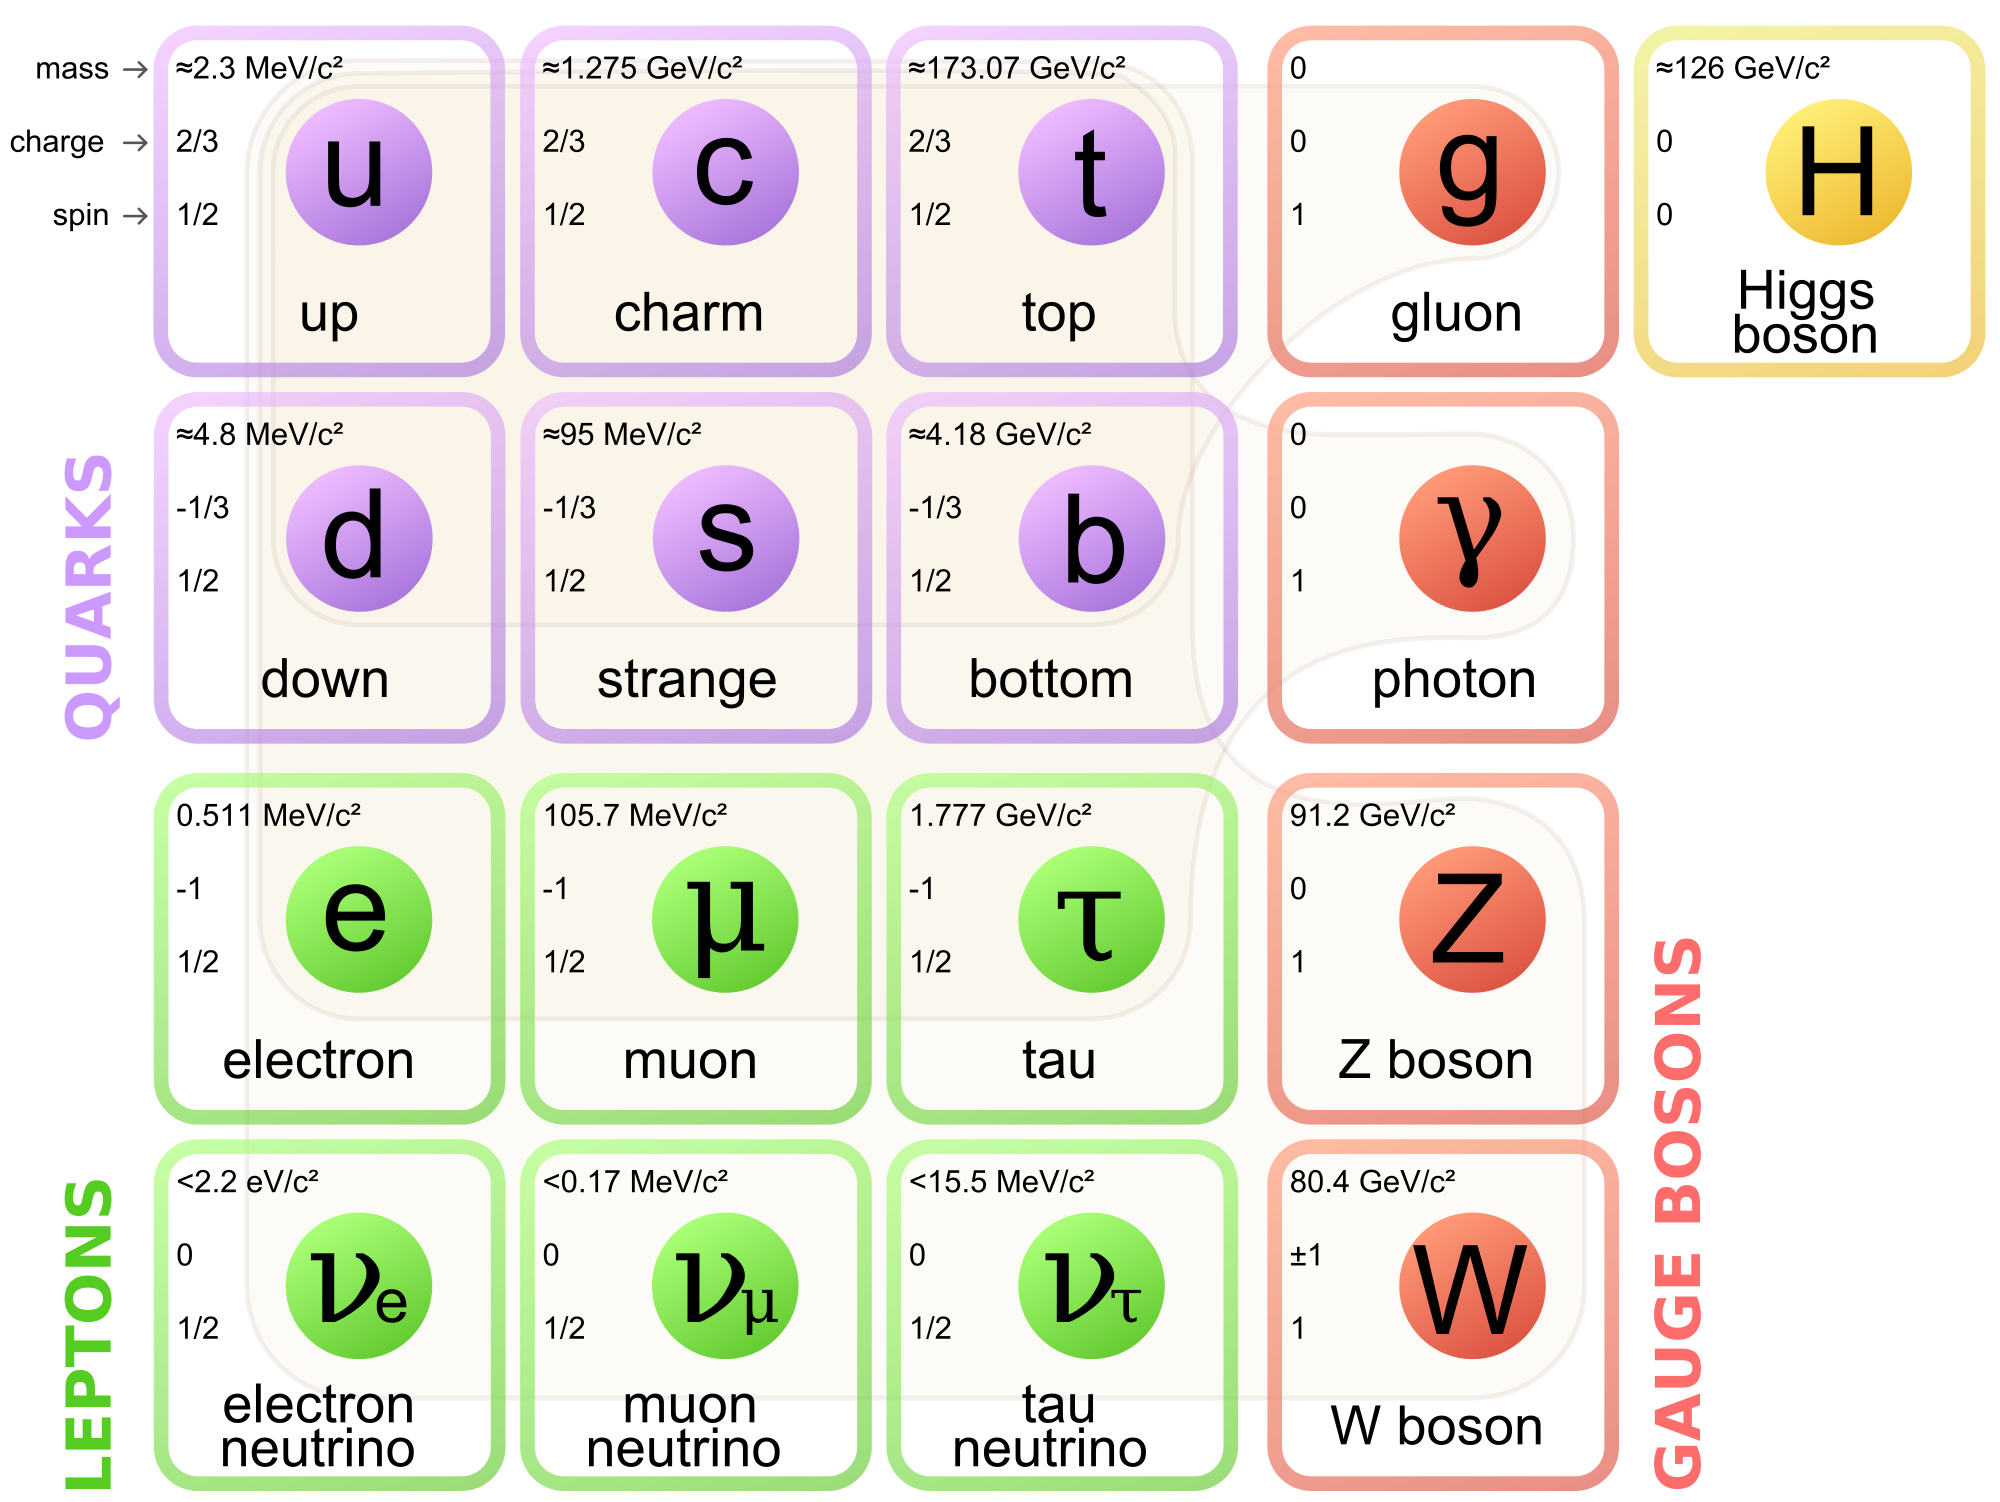
\includegraphics[width=.7\textwidth]{figures/Standard_Model_particles.png}
\caption{Standard model of elementary particles: 
the 12 fundamental fermions and 5 fundamental bosons.~\cite{particleImage}}
\label{figs:SMParticles}
\end{figure}  

%\subsection{Weak interactions of quarks}

%The charged weak interaction of quarks doesn't obey the "generation-conservation laws" of 
%leptonic weak interactions, which means W boson could decay to u, d quarks, while W 
%could also decay to u, s quarks.  

%{\bf CKM matrix}

\section{Fundamental interactions}

In SM, there are four fundamental forces : strong, electromagnetic,  weak and 
gravitational force, as shown in Table~\ref{table:fourForces}. The ``Strength'' column 
in Table~\ref{table:fourForces} is not the real strength of the force, 
but a value to show the relative strength of these forces. 
 
Since gravity is so small compared to other three forces, it is mostly not considered in 
the process of particle physics. 
The theory of particular interest to my thesis 
is the QCD, which will be introduced in the following section.  
 %Here in this section, the other three forces 
 %will be introduced.  Feynman diagrams will be used to help understanding the 
 %theories. 
 % Here I will assume the readers have basic knowledge of Feynman diagrams. 
 %Details about Feynman diagrams could be found in Ref.~\cite{feynman}

\begin{table}
\begin{tabular}{cccc}
Force & Strength & Theory & Mediator \\
\hline 
Strong  & 10 &  Quantum Chromodynamics  & Gluon \\
Electromagnetic & $10^{-2}$ & Quantum Electrodynamics & Photon \\
Weak & $10^{-13}$ & Flavordynamics & W and Z \\
Gravitational & $10^{-42}$ & Geometrodynamics & Graviton \\
\hline 
\end{tabular}
\caption{Summary of the four fundamental forces in Standard Model~\cite{particlebook1}.}
\label{table:fourForces}
\end{table} 



%Here in this section, we will briefly introduce the Quantum Electrodynamics (QED),  

%\subsection{Quantum Electrodynamics (QED)}

%The basic ``naive" process in QED, as shown in Figure~\ref{fig:basicFeyman}, is that
%an electron comes in, then radiates a photon and goes out. 
%It could 
%never happen standalone, because this againsts energy and momentum conservation. 
%However,  all other processes in QED could be built by this ``naive" process.  For example, 
%the BaBa scattering and Moller scattering, as shown in Figure~\ref{fig:baba} and ~\ref{fig:moller}. 


%\begin{equation}

%\end{equation}

 
%\subsection{}

%\subsection{W, Z and Higgs}


\subsection{Quantum Chromodynamics (QCD) and jets}

QCD is a theory describing the strong force and the involved fundamental particles. 
As we see from Table~\ref{table:fourForces}, strong force is the strongest force of the four. 
However, unlike the long range electromagnetic force, 
the strong force could only affect ${\approx} 10^{-15}m$ (1fm), which is about the radius of 
a nuclei. 

Color is one of the unique properties of QCD. One could think of color of QCD as an analogy to the charge of QED. Note it is just a property label, not the same color we use in daily life. 
There are three types of colors, as we mentioned earlier, red,
blue, green. Each quark carry one kind of color. 
Anti-quark carries one kind of anti-color.  Gluons has a mixture of color. 
So when two quarks interacts with each other, 
they interacts through a gluon by exchanging colors.
For example, one blue quark comes in, and radiates a gluon with color blue and anti-red, 
then a red quark goes out.  
Gluons is the boson intermediating the strong force, just like the fact that
photon is the mediator of the electromagnetic force.

Unlike charge particles, colored particle could not be free. What we see in experiments and daily life is 
color-neutral, or more precisely color-singlet. So we can never observe a single quark or a single gluon 
in experiment. What we observes is the hadronization product of quarks and gluons, which are
called jets. The existence of quarks and gluons is proved by indirect experiments via jets. 
Here we will introduce the essential components of QCD. 
%However, we can prove their existence by some other indirect measurements. 
%{\color{red} Here I might want to cite some experiment}

{\bf The coupling constant}

Coupling constant is the number describing the strength of an interaction. 
Here in QCD, the coupling constant $\alpha_{s}$ is :
\begin{equation}
\alpha_{s}(|q^2|) = \frac{2\pi}{(11n-2f)ln(|q^2|/\Lambda^2)}   \quad (|q^2| \gg \Lambda^2)
\label{equation:coupling}
\end{equation}
where  $|q|^2$ is the squared energy-momentum 4-vector of the mediator gluon, $n$ is the number of colors (3, in SM), 
$f$ is the number of flavors (3, in SM), and $\Lambda$ is a parameter determined from 
experimental data, which is in the range of $100 {\sim} 500$~MeV. 

Notice that $\alpha_{s}$ is not a constant. It is a function of $|q|^2$. Because of this, it is also 
named the "running coupling constant".  The experimental measurements are shown 
in Figure~\ref{figs:coupling}

\begin{figure}[htb]
\centering
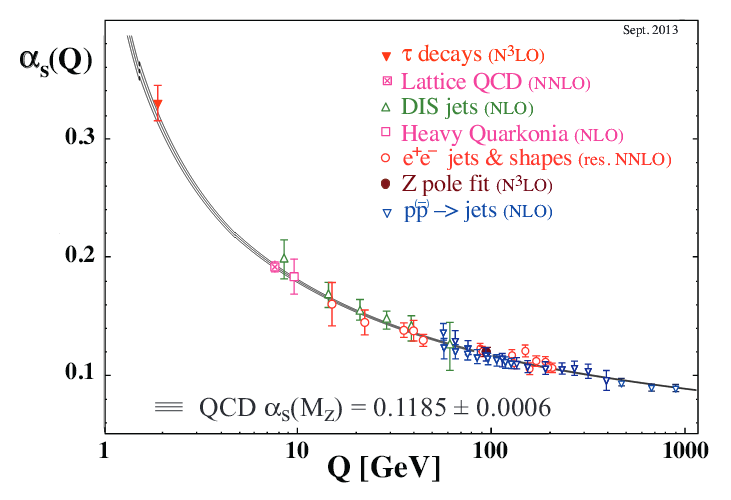
\includegraphics[width=.7\textwidth]{figures/alphasrunning.png}
\caption{The running coupling constant of QCD. }
\label{figs:coupling}
\end{figure}  

 
{\bf Asymptotic freedom}

As we see from Equation~\ref{equation:coupling}, 
when $|q|^2$ increases, $\alpha_{s}$ will decrease. 
At short distances (${\leq}1~fm$), and also large $|q|^2$, the strong force 
is so weak that quarks inside of proton travel freely.  At very high energies, 
it is also possible to form quark-gluon plasma, since their interactions are so weak. 
This is called the asymptotic freedom. 

{\bf QCD confinement}


QCD confinement means that the force between quarks will hugely increase when they are separated. 
So one has to exert a lot energy to try to separate a quark from other quarks. And this energy will
become large enough for the mediator gluon to decay into a new quark pair. 
As illustrated in Figure~\ref{fig:color_field},  when the two charm quarks are pulled apart, the 
strong force between them will increase, which means the mediating gluon will have 
a huge amount of energy. Before the charm quarks are further separated, the gluon will 
decay to a pair of d quarks. And eventually the particle formed by two charms quarks will become 
two particles each formed by c and d quarks. The gluon could decay to any pair of new quarks, 
as long as the energy is large enough to create them. Here we use d quarks pair as illustration. 
And also d quark pairs require relatively small energy to create. 

\begin{figure}[htb]
\centering
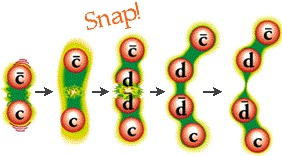
\includegraphics[width=.7\textwidth]{figures/color_field.jpg}
\caption{The illustration of QCD confinement~\cite{web:qcd_confinement}.}
\label{fig:color_field}
\end{figure}  



{\bf Jet formation}

In the particle collider, when two particles collide with each other, the resulting quarks and 
gluons (if created) will travel freely for a brief moment with large energy. And then because of 
QCD confinement, when the ``free" quarks are separated by distance ${\geq} 1fm$, 
these quarks will radiates gluons, which further decay to new quark pairs. 
This process will not stop until the gluons or quarks don't have enough energy to 
create new quark pairs. So the initial created quarks or gluons will 
eventually become hadrons, and this process is called hadronizaiton, as shown
in Figure~\ref{fig:hadronization}. 
The tight cone of particles created by 
the hadronization of a single quark or gluon is called a jet, as shown in 
Figure~\ref{fig:hadronization}

\begin{figure}[htb]
\centering
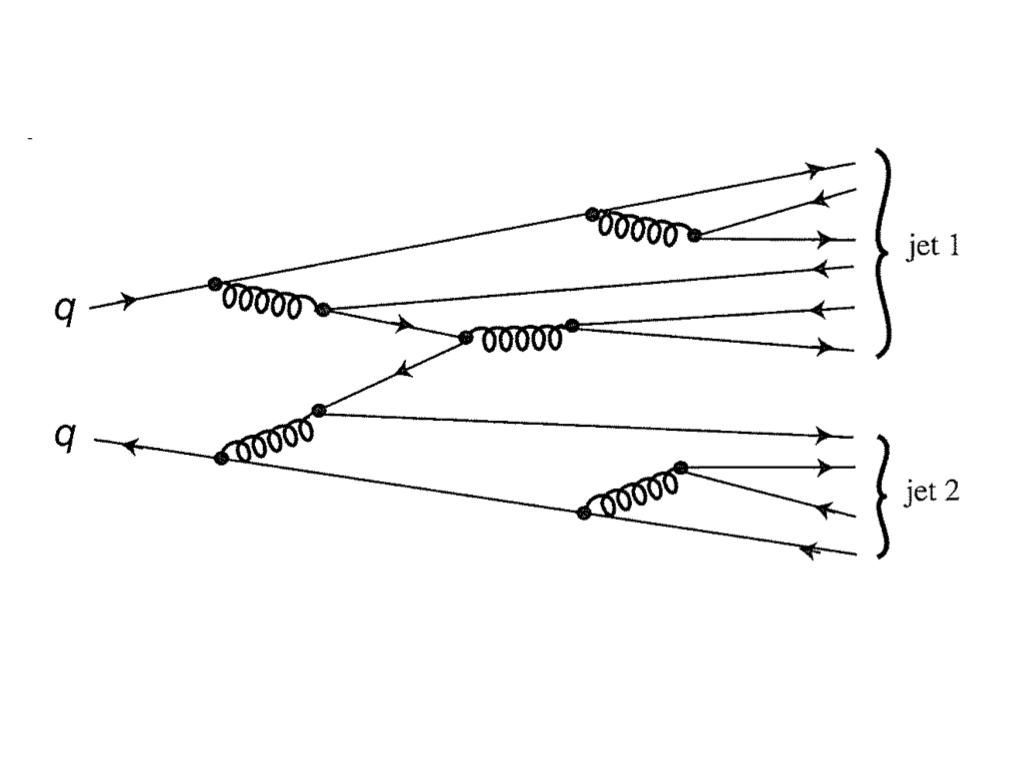
\includegraphics[width=.7\textwidth]{figures/jets.png}
\caption{The hadronization process~\cite{particlebook1}.}
\label{fig:hadronization}
\end{figure}  

\begin{figure}[htb]
\centering
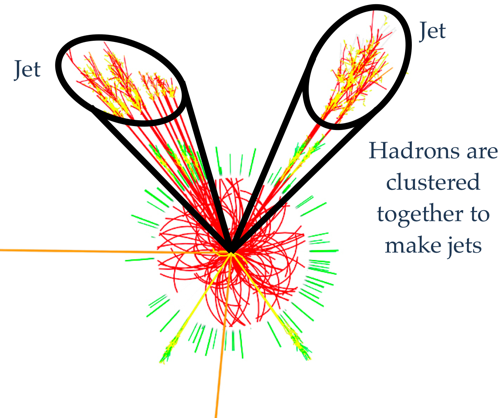
\includegraphics[width=.7\textwidth]{figures/clustering.png}
\caption{Jets formation.}
\label{fig:jet_formation}
\end{figure}  

%\subsection{Charged weak interaction of quarks: CKM matrix}


%\subsection{The SM Higgs boson}

%The SM Higgs boson is coming through the electroweak symmetry breaking 
%mechanism in SM, accounting for the mass of W, Z and also the all the fermions. 







%The connection between symmetries and physics is deep. Noether's theorem states, essentially, that for every continuous symmetry of Nature there is a corresponding conservation law. 
%The construction of the Standard Model has been guided by principles of symmetry and also 
%symmetry breaking. 
\section{The physics beyond the SM}

Although the SM explains a lot of facts of current experiments and also achieves another tremendous success on 
the discovery of the SM-like Higgs boson in 2012. However, It is not perfect. 

{\bf Dark matter and dark energy}

``More is unknown than is known" (quoted form NASA website). 
As shown in Figure~\ref{fig:universe}, the universe is expanding, instead of slowing down,
but acceleratedly. 
Based on Newton's second law, $F = ma$, there must be some mysterious force 
causes the expansion and is bigger than the attractive force of gravity. 
For the source of this unknown force, we name it "dark energy". Dark here is 
the thing invisible to us. 

The needs for dark matter arises from the astronomy observations that the rotational motion of 
the stars or galaxies suggests a $5{\sim}10$ times larger gravitational force than the one could be provided 
by the matter of the clusters. The lack of matter in this kind of case indicates the existence of 
matter that couldn't be observed by us, which we name it ``dark matter".   
 
In the current study,  the constituents of matter and energy of our universe are about 4.9\% normal matter (like earth, sun, etc.), 26.8\% dark matter, and 68.3\% dark energy. Although in SM, neutrinos, which has tiny mass and interacts weakly with other particles, behave like 
the dark matter. However, the redundancy of dark matter (26.8\%) over normal matter (4.9\%) suggests that neutrinos are far from enough. 

\begin{figure}[htb]
\centering
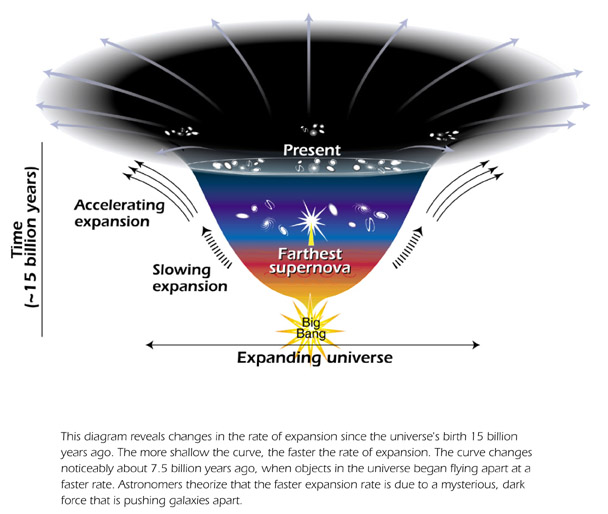
\includegraphics[width=.7\textwidth]{figures/accelerating_universe.jpg}
\caption{Accelerating expansion of the universe~\cite{web:nasa}.}
\label{fig:universe}
\end{figure}  



{\bf The hierarchy problem}

As shown in Table~\ref{table:fourForces}, the gravitational force is quite small compared 
to other three forces. It is about $10^{-30}$ smaller than the weak force. This is the 
hierarchy problem. 
The more formal way to state the hierarchy problem is why the Higgs mass in SM is in the scale of
${\approx}125$ GeV, 
rather not $10^{18}$ GeV, while the latter is more natural. 

The hierarchy problem arises from the fact that as a scaler particle, with zero spin, the Higgs 
mass calculation using Feynman diagrams will eventually break down (divergent integral), which 
suggests Higgs particle possesses a large mass, about the Planck mass scale ($10^{18}$~GeV), which is the 
energy scale where our theory breaks down. 
However, in SM, Higgs boson accounts for the mass of W, Z, and all the fermions, through the 
mechanism of electroweak symmetry breaking. Although not confined, 
the SM H mass is preferably to be around $100$~GeV-ish, to account for 
the scattering process of longitudinally polarized vector bosons.  

%The recent discovered SM-like Higgs boson has a mass ${\approx} 125$~GeV, which 


{\bf The graviton}

 Graviton is the mediator for gravitational force in SM. However, it has not been found yet. 
 Unlike the QED and QCD, there is no known way to explain relativity in SM. 
 \\
 \\
 Since SM leaves us a lot of mysteries,  the scientific research towards a better understanding of 
 our universe has never been stopped. In this thesis, two searches for physics beyond the SM are 
 conducted. 
 





